Este capítulo é onde começamos a abordar nosso modelo proposto de um sistema de arquivos distribuídos tolerante a falhas. Iniciamos com um visão geral da arquitetura do sistema apresentando detalhes do serviço de metadados, serviço de armazenamento,, servidor e do cliente. Em seguida é abordado as operações realizadas pelo sistema de arquivos distribuído proposto, tais operações estão divididas entre operações do tipo Cliente-Servidor e Servidor-Servidor. Seguindo com o capítulo, é explanado como foi realizada a implementação do sistema de arquivos distribuído utilizando conceitos de RAID proposto, focando especialmente nos serviços de metadados e de armazenamento, além dos clientes. Enfim, o capítulo finaliza apresentado o planejamento e execução dos experimentos seguido da análise dos dados obtidos.


	\section{Arquitetura do sistema}
	
	A arquitetura do Sistema de Arquivos Distribuídos proposto neste trabalho é composto por um ou vários clientes comunicando-se com ao menos três servidores de metadados e quatro servidores de armazenamento, onde cada um deles está conectado através de Internet ou outra rede, como a Figura~\ref{fig:vis_sis}  sintetiza. Neste sistema, cada servidor de armazenamento se comporta como um disco rígido em sistema de RAID, armazenando distribuidamente as partes dos arquivos e/ou paridades associadas. \\
	
	
	%O nosso objeivo neste artigo é a construção de um SAD baseado na computação em nuvem que possui menor \textit{overhead} de espaço, comparado a 200\% de método de replicação, sem degradar muito o performance e segurança de dados. 
	%Para isso, nós observamos em técnica de redundância usado na tecnologia RAID, onde consegue diminuir o espaço ocupado pela parte redundante com atribuição de paridade nos arquivos, ao invés de simples replicação. Na mesma tecnologia também foi 

	
	
	\begin{figure}[htb]
		\begin{center}
			
			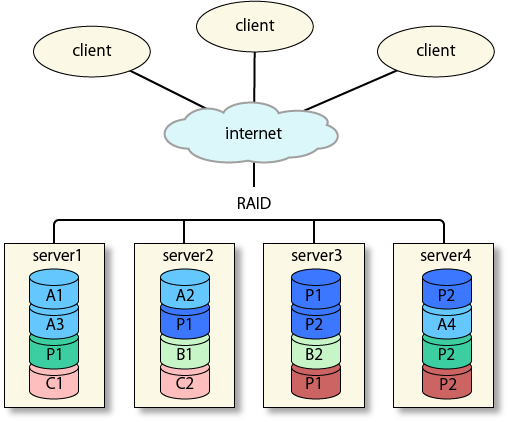
\includegraphics[clip,width=10.0cm]{images/image1.png}
			\caption{Visão geral do sistema}
			\label{fig:vis_sis}
		\end{center}
	\end{figure}
	
	Em um sistema de arquivos local, normalmente o metadado e o conteúdo de um arquivo são armazenados na mesma unidade de armazenamento. No caso de um SAD, como um arquivo pode ser armazenados distribuidamente entre servidores diferentes, os metadados são espalhados por vários servidores, tendo assim, a necessidade de fazer a busca para acessar em um determinado metadado. Obviamente essa busca consome recursos operacionais, relativamente alta por tratar de uma transmissão na rede.   \\
	
	\begin{figure}[htb]
		\begin{center}
			
			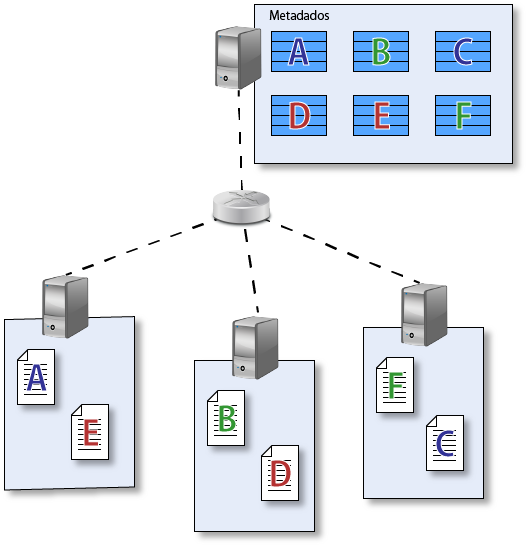
\includegraphics[clip,width=10.0cm]{images/image7.png}
			\caption{\textit{Name node} e \textit{data node}}
			\label{fig:namenode}
		\end{center}
	\end{figure}
	
	\subsection{Serviço de Metadados}
		Grupo de servidores que fazem o gerenciamento dos dados.\\
		
		Em nosso sistema utilizamos o conceito de blocos, onde um bloco é um conjunto de dados de um dado arquivo ou os dados de paridade de um determinado arquivo. O tamanho do bloco é determinado levando em consideração a quantidade de servidores de armazenamento ativos, ou seja, se houverem quatro servidores ativo, então o arquivo (independente de seu tamanho) será dividido em quatro blocos de tamanhos idênticos, caso seja necessário, o ultimo bloco será preenchido com bits '0' até que o bloco alcance o tamanho previamente fixado.
		\\ 
		
		O Serviço de metadados, também conhecido por \textit{name node}, é o conjunto de servidores que gerencia as informações dos arquivos armazenados, utilizando-se dos metadados. Em nosso sistema a data de criação, data da ultima modificação, data do ultimo acesso, tamanho, identificador do bloco de dados e nome do servidor são considerados metadados. 
		\\
		
		É da responsabilidade do sistema de metadados gerenciar a comunicação entre cliente e servidores de armazenamento (ou  \textit{data nodes}), utilizando-se das informações que indicam  estado atual do sistema e qual o tipo de RAID está sendo utilizado (apenas um tipo de RAID pode ser utilizado por operação) o \textit{name node} deve decidir em quantos blocos de tamanho idêntico o arquivo deve ser dividido e em quais servidores de armazenamento cada bloco deve ser armazenado.
		\\ 
		
		Nosso sistema está preparado para tratar os seguintes tipos de RAID, os quais foram explorados com maior profundidade no capítulo 4.
		\\
		
		\begin{itemize}
			\item RAID 0 - fracionamento simples;
			\item RAID 1 - espelhamento;
			\item RAID 5 - fracionamento com paridade espalhada entre os discos do vetor.
		\end{itemize}
		
		O Serviço de metadados mantém na sua memória local a árvore de diretórios, o que indica localização lógica dos arquivos. Quando recebe uma solicitação de cliente por um arquivo, pesquisa a sua árvore de diretórios para identificar qual diretório que este arquivo se encontra. Como resultado da pesquisa obtém o metadado do arquivo referente, conseguindo descobrir a sua localização física, a lista dos todos os \textit{data nodes} que possuem as partes do arquivo.
		\\
		
		Por sua propriedade como um interface entre clientes e \textit{data nodes}, a ocorrência de alguma falha na operação ou indisponibilidade causada pela queda do servidor tem  enorme influencia na execução do sistema, podendo até resultar em parada total do sistema. Assim, é muito importante elaborar uma esquema para manter o \textit{name node} protegidos contra falhas ou queda total. Em nosso sistema usaremos a biblioteca BFT-SMaRt, que fornece tolerância a falha no serviço através de replicação por máquina de estado. \\
	
	\subsection{Serviço de Armazenamento}
		Grupo de servidores que fazem armazenamento físico dos dados gerenciados pelo sistema de metadados. Também conhecidos como \textit{data nodes}.\\
		
		Em nosso sistema, o serviço de armazenamento não possui a necessidade de saber qual tipo de RAID está sendo executado, a responsabilidade de manter o RAID consistente é toda do serviço de metadados. Desta forma, o sistema de armazenamento apenas se conecta a uma porta e fica aguardando algum cliente se conectar a sua respectiva porta. Quando algum cliente conecta-se na porta do servidor, é realizado um \textit{handshake} preliminar, logo em seguida o cliente inicia a transferência dos dados que devem ser guardados pelo sistema de armazenamento. Ao fim da transferência o cliente fecha a conexão, enquanto o sistema de armazenamento indexa o arquivo recebido utilizando as informações adicionais que o serviço de metadados anexou ao arquivo. Com tais informações é possível saber o identificador tanto do arquivo quanto do cliente que o enviou. Tais dados adicionais são necessários para garantir que apenas o usuário dono dos dados enviados tenha acesso a eles, além de possibilitar identificar quais dados o cliente deseja receber de forma simples e eficiente.  
		\\
	
	\subsection{Cliente}
	O programa cliente executado no computador de um usuário do sistema. 
	\\
	
	Para cada operação que deseje realizar, o programa cliente (doravante Cliente) deve primeiramente comunicar-se com o serviço de metadados o qual ou irá realizar a operação (no caso de operações envolvendo diretórios) ou informar com quais servidores de armazenamento o cliente deve se comunicar e quais blocos devem ser enviados para cada servidor. Entretanto, é função do Cliente informar qual tipo de RAID ele deseja utilizar.
	\\
	
	O programa cliente é capaz de dividir um arquivo em vários pedaços e gerar paridades. Por consequência, também é capaz de reconstruir um arquivo a partir de partes divididos. A Figura~\ref{fig:img6} mostra o procedimento.
	\begin{figure}[htb]
		\begin{center}
			
			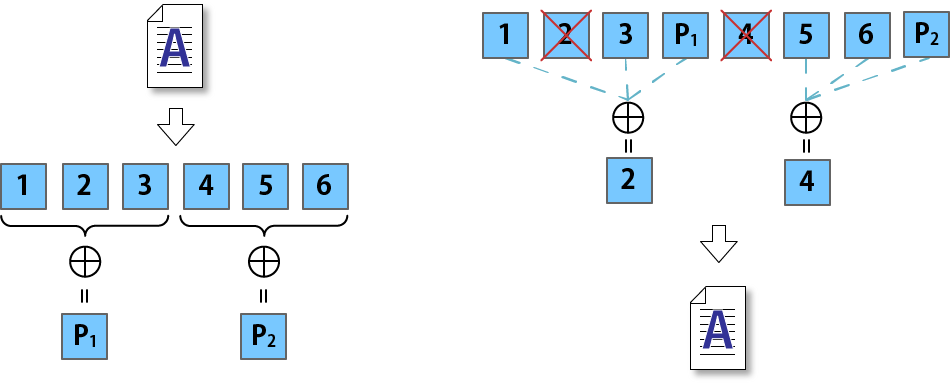
\includegraphics[clip,width=15.0cm]{images/image6.png}
			\caption{Geração de paridade}
			\label{fig:img6}
		\end{center}
	\end{figure}
	
	Para assegurar a disponibilidade do sistema, é interessante que o usuário tenha acesso ao um arquivo mesmo que algum dos seus fragmentos de dado esteja indisponível por uma razão qualquer, recuperando o arquivo íntegro a partir de fragmentos disponíveis neste momento.\\
	
	Quando um cliente percebe que o arquivo que solicitou apresenta  
	A Figura~\ref{fig:img2} mostra esquema para recuperar um arquivo no lado do cliente.
	
	\begin{figure}[htb]
		\begin{center}
			
			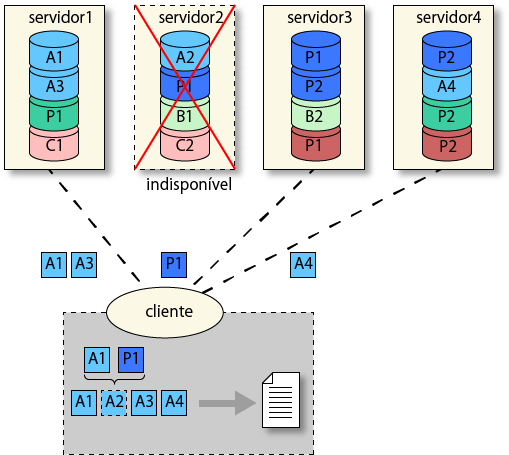
\includegraphics[clip,width=10.0cm]{images/image2.png}
			\caption{Recuperando um arquivo de uma falha}
			\label{fig:img2}
		\end{center}
	\end{figure}
	
	\section{Operações no Sistema de Arquivos Distribuídos}
	
	Nesta seção serão apresentadas as operações básicas que o SAD executa. Estas operações podem ser divididos em dois grupos dependendo dos entidades envolvidos na operação executada. Um deles é entre cliente e servidor, onde consiste das operações que podem ser encontradas em sistemas de arquivos em geral, focalizadas em fornecer um serviço de armazenamento de dados. Outro tipo é as operações que ocorrem entre servidores, voltadas para gerenciamento do serviço. Este tipo de operação não pode ser percebido por usuário, mantendo algumas transparências.
	
	
	%Os protocolos neste sistema indicam os tipos de mensagens que vai ser trocado entre cliente/servidor ou servidor/servidor. 
	
	\subsection{Cliente-Servidor}
	
	É um conjunto de operações semelhantes a que são implementadas em um sistema de arquivos local, aquele que é integrado na maioria dos sistemas operacionais comuns. Composto pelas operações sobre arquivos e pastas e suas execuções podem ocorrer entre cliente e \textit{name node} ou cliente e \textit{data node}.
	
	\subsubsection{Criar arquivos}
	
	Quando um cliente deseja criar um arquivo dentro de um SAD, primeiramente deve enviar para servidor do tipo \textit{name node} o metadado referente ao arquivo, o que contem as informações essenciais como nome, diretório, tamanho e entre outros. No lado do servidor, recebendo o metadado do arquivo a ser criado, extrai dele o nome e diretório do arquivo. 
	
	\subsubsection{Abrir arquivos}
	
	Abrir um arquivo existente provavelmente vai ser uma das tarefas mais usado no sistema. Geralmente é composto por três procedimentos básicos. Esta operação inicia pegando como referencia o nome e o diretório do arquivo, e procura por nome neste diretório. É muito importante que a busca pelo arquivo tenha uma boa eficiência, pois uma vez que este procedimento é executado muitas vezes e normalmente um servidor de grande porte possui  diretórios com milhares entradas encontrados dentro deles. Assim, a escolha do estrutura de dados para diretórios pode influenciar criticamente no desempenho do sistema. Depois de encontrar o arquivo desejado, será verificado algumas condições para decidir se o arquivo pode ser aberto mesmo. Uma condição é se o arquivo não esteja bloqueado por outros usuários, impedindo que seja aberto no momento. Outra é se o usuário que solicitou o acesso por este arquivo possui a permissão para fazer isso. Passando por checagem das permissões de acesso, finalmente o servidor envia uma resposta para cliente, indicando os servidores que armazenam cada pedaços do arquivo.
	 
	\subsubsection{Deletar arquivos}
	Deletar um arquivo vai seguir procedimentos semelhantes a operação de abrir arquivo. Em primeiro lugar recebe o nome e diretório do arquivo a ser apagado. Faz a busca pela árvore de diretórios para achar o diretório requisitado, e chegando em diretório correto, procura o arquivo por nome. Quando encontra o arquivo desejado, verifica se está satisfazendo as condições para efetuar a operação, checando a permissão de acesso e estado de bloqueio do arquivo.  
	
	\subsubsection{Fechar um arquivo aberto}
	
	Fechar o arquivo aberto por um cliente.
	
	\subsubsection{Editar um arquivo}
	
	Fazer alteração no arquivo armazenado.
	
	\subsubsection{Modificar metadado}
	
	Permite fazer alterações sobre as informações do arquivo, editando diretamente o metadado associado.
	
	
	\subsection{Servidor-Servidor}
	São operações ocorridos entre \textit{name node} e \textit{data node}, com função de gerenciamento de SAD.
	
	\subsubsection{Receber arquivo criado}
	
	Na operação de criar arquivo, o \textit{name node} define quais \textit{data nodes} vão ser utilizados para armazenar os fragmentos de arquivo a ser criado, calculando a melhor forma para distribuir igualmente a carga entre os \textit{data nodes}. Dessa forma, além de informar o cliente quais são os servidores que deve enviar os dados, deve avisar os \textit{data nodes} que vai chegar dados enviados pelo cliente.
	
	\subsubsection{Apagar arquivo deletado}
	
	Deleta os dados pertencentes ao arquivo solicitado para exclusão.
	
	\subsubsection{Transferir dados entre servidores}
	
	Transferência de arquivos entre \textit{data nodes}.
	
	
	\section{Implementação}
	
	\subsection{Serviço de Metadados}
	
	\subsection{Serviço de Armazenamento}
	
	\subsection{Cliente}
	
	
	\section{Experimentos}
	
	\section{Conclusões do Capítulo}
	
	
	